\section{Logik}
\lecdate{10.10.2017}
\subsection{Aussagen und Wahrheitswerte}

\paragraph{1. Definition} \parskp
Eine Aussage ist ein aus W"ortern und/oder mathematischen Zeichen aufgebauter Ausdruck, bei dem es m"oglich und sinnvoll ist zu entscheiden, ob dieser Ausdruck \enquote{wahr} oder \enquote{falsch} ist.

\paragraph{2. Bemerkung}
\begin{itemize}
	\item Wahrheitsgehalt \true mit \enquote w oder \enquote 1 abgek"urzt
	\item Wahrheitsgehalt \false mit \enquote f oder \enquote 0 abgek"urzt
	\item Typische Bezeichnungen f"ur Aussagen sind $a$, $b$, $c$, \dots
	\item Tats"achlich gibt es in der Mathematik Aussagen, die nicht entscheidbar sind (weder \true noch \false)
\end{itemize}

\paragraph{3. Beispiel}
\begin{enumerate}
	\item Es gibt unendlich viele Primzahlen (\tgreen{\true})
	\item Es gibt unendlich viele Primzahlzwillinge (\tgrey{Aussage mit unbekanntem Wahrheitswert})
	\item $5+7=13$ (\tred{\false})
	\item Wie sp"at ist es (\tgrey{keine Aussage})
	\item Diese Aussage ist falsch (\tgrey{keine Aussage, da keine sinnvolle Entscheidung m"oglich})
	\item Am 24.12. wird es schneien (\tgrey{Aussage mit unbekanntem Wahrheitswert})
\end{enumerate}

\paragraph{4. Definition} Die Negation einer Aussage ist genau dann wahr, wenn $a$ falsch ist.\\
Bezeichnung: $\bar a, \neg a$\\
Darstellung der Negation:  $\begin{array}{l|l}
	a & \bar a\\\hline
	0 & 1\\
	1 & 0
\end{array}$

\subsection{Verkn"upfung von Aussagen}

Wir definieren Verkn"upfungen von Aussagen durch die Angabe der Wahrheitstabelle
\begin{enumerate}[label=\alph*)]
	\item Konjunktion $a\land b$
	\item Disjunktion $a\lor b$
	\item Implikation $a\To b$\\
	$a$\dots Premisse \quad $b$\dots Konklusion\\
	Eine Implikation ist dann falsch, wenn die Premisse richtig ist und die Konklusion falsch ist. $\neg a\lor b$\\
	\begin{align*}
		\text{\underline{Beispiel:} } -1=1\text{ (falsch)}&\xRightarrow{sqrt}1=1\text{ (wahr)}\\
		-1=1\text{ (falsch)}&\xRightarrow{+1}0=2\text{ (falsch)}
	\end{align*}
	Aus einer falsche Aussage lassen sich durch richtiges Schlie"sen sowohl falsche Aussagen, als auch richtige Aussagen erzeugen.
	\item "Aquivalenz $a\Leftrightarrow b$\\
	$a\Leftrightarrow b$ ist gleichbedeutend mit $(a\To b)\land(b\To a)$\\
	Wir nutzen $:\Leftrightarrow$ um Aussagen zu definieren bzw. um verkn"upften Aussagen eine neue Bezeichnung zu geben $c:\Leftrightarrow(\bar a\land b)$
\end{enumerate}
$\begin{array}{c|c|c|c|c|c}
	a & b & a\land b & a\lor b & a\To b & a\Leftrightarrow b \\\hline
	0 & 0 & 0 & 0 & 1 & 1 \\
	0 & 1 & 0 & 1 & 1 & 0 \\
	1 & 0 & 0 & 1 & 0 & 0 \\
	1 & 1 & 1 & 1 & 1 & 1
\end{array}$

\subsection{Logische Gesetze (Tautologien)}

Eine Tautologie ist eine Aussagenverbindung/Verkn"upfung, die unabh"angig vom Wahrheitswert der einzelnen Aussage stets \true ist.
\begin{enumerate}[label=\alph*)]
	\item $a\Leftarrow \bar{\bar{a}}$ (Negation der Negation)
	\item $a\lor a$ (Satz vom ausgeschlossenen Dritten)
	\item $(\overline{a\land b})\Leftrightarrow\bar a\lor \bar b$ (de Morgansche Regel)\\
	$(\overline{a\lor b})\Leftrightarrow\bar a\land \bar b$ (de Morgansche Regel)
	\item $(a\To b)\Leftrightarrow\bar b\To\bar a$ (Kontrapositionsgesetz)
	\item $(a\To b)\Leftrightarrow\bar a\To b$
	\item $(a\land(a\To b))\To b$ (direkter Beweis)
	\item $(a\land(\bar b\To\bar a))\To b$ (indirekter Beweis)
\end{enumerate}
Beweis mittels Wahrheitstafeln, siehe "Ubung 1\\
Beachte: Eine "Aquivalenz ist eine Tautologie \gdw die Wahrheitswerte beider Seiten "ubereinstimmen.

\lecdate{11.10.2017}
\paragraph{6. Bemerkung (Beweistechniken)} Zu beweisen ist $b$
\begin{enumerate}
	\item Direkter Beweis
	\begin{itemize}
		\item Nachweis/Annahme von $a$ (Voraussetzung)
		\item Nachweis, dass die Implikation $a\Leftrightarrow b$ gilt\\
		Dann ist b wahr (Behauptung)
	\end{itemize}
	\item Indirekter Beweis
	\begin{itemize}
		\item Nachweis/Annahme von $a$ (Voraussetzung)
		\item Annahme von $\bar b$ auf Widerspruch f"uhren (z.B. Nachweis, dass $\bar a$ gilt)\\
		Dann ist b wahr (Behauptung)
	\end{itemize}
\end{enumerate}

\paragraph{7. Beispiel} $a:\Leftrightarrow$, Eine Zahl ist rational, wenn sie als Bruch teilerfremd ganzer Zahl geschrieben werden kann.\\
$b:\Leftarrow$, $\sqrt{2}$ ist irrational\\
\\
Zu zeigen ist $b$. Voraussetzung ist $a$\\
Beweis (indirekt):\\
Es gelte $\bar b$, d.h. $\sqrt{2}$ ist rational. Dann gelten folgende Schl"usse
\begin{align*}
	a&\To\sqrt{2}\To\frac{m}{n}\text{ mit teilerfrenden Zahlen }n\text{ und }m\\
	&\To2=\frac{m^2}{n^2}\To2\cdot n^2=m^2\\
	&\To2|m^2\text{ (}2\text{ ist Teiler von }m^2\text{)}\\
	&\To2|m\\
	&\To4|m^2\text{ (mit }m^2=2n^2\text{)}\\
	&\To4|2n^2\\
	&\To2|n^2\\
	&\To2|n\\
	&\To n\text{ und }m\text{ sind keine teilerfrenden Zahlen, da }2|m\text{ und }2|n\To\text{ Widerspruch}
\end{align*}
Weitere Gesetze:
\begin{enumerate}[label=\alph*)]
	\item $(a\land b)\Leftrightarrow(b\land a)$ (Kommutativgesetz)\\
	$(a\lor b)\Leftrightarrow(b\lor a)$
	\item $((a\land b)\land c)\Leftrightarrow(a\land(b\land c))$ (Assoziativgesetz)\\
	$((a\lor b)\lor c)\Leftrightarrow(a\lor(b\lor c))$
	\item $a\land(b\lor c)\Leftrightarrow(a\land b)\lor(a\land c)$ (Distributivgesetz)\\
	$a\lor(b\land c)\Leftrightarrow(a\lor b)\land(a\lor c)$
	\item $a\land1\Leftrightarrow a\qquad a\land0\Leftrightarrow0$\\
	$a\lor1\Leftrightarrow1\qquad a\lor0\Leftrightarrow a$\\
	$a\lor a\Leftrightarrow a\qquad a\lor a\Leftarrow a$
	\item $a\lor(a\land b)\Leftrightarrow a$ (Absorbtionsgesetz)
\end{enumerate}

\subsection{Aussagefunktionen, Quantoren, Pr"adikatenlogik}
$X$ sei eine Menge (Gesamtheit von bestimmten wohlunterschiedenen Objekten) $x\in X$. Die Objekte haben Eigenschaften (Pr"adikaten)

\paragraph{8. Definition} (Aussagefunktion bzw. Aussageform)\\
Ist $a(x)$ f"ur jedes $x\in X$ eine Aussage, so nennt man die Funktion $a:X\to\{\text{wahr, falsch}\}$ eine \underline{Aussagefunktion} bzw. \underline{Pr"adikat} bzw. \underline{Aussageform}.

\paragraph{9. Beispiel} $X$\dots Menge der nat"urlichen Zahlen 
\begin{itemize}
	\item $a(x):\Leftrightarrow$ \enquote{$x$ ist eine Primzahl}
	\item $a(5)$ \tgreen{\true}
	\item $a(4)$ \tred{\false}
\end{itemize}

\paragraph{10. Definition} Ist eine Aussagefunktion $a$ f"ur Elemente von $X$ gegeben, do nutzten wir folgende Kurzschreibweise:
\begin{enumerate}[label=\alph*)]
	\item \enquote{F"ur alle $x\in X$ gilt $a(x)$}\\
	$\Leftrightarrow:\forall x:a(x)$ (universeller Quantor, Allquantor)
	\item \enquote{Es existiert mindestens ein $x$, f"ur welches $a(x)$ gilt}\\
	$\Leftrightarrow:\exists  x:a(x)$ (existenzieller Quantor, Existenzquantor)
	\item \enquote{Es existiert genau ein $x$, f"ur welches $a(x)$ gilt}\\
	$\Leftrightarrow:\exists!x:a(x)$ (Eindeutigkeitsquantor)
	\item \enquote{Es existiert kein $x$, f"ur welches $a(x)$ gilt}\\
	$\Leftrightarrow:\nexists x:a(x)\Leftarrow\forall x:\overline{a(x)}$
\end{enumerate}

\paragraph{11. Bemerkung} Bei Anwendung (au"serhalb der reinen Logik) wird oft die Grundmenge mit angegeben. $\forall x\in X:a(x)$
\begin{itemize}
	\item Falls sich Quantoren auf eine Teilmenge $M$ von $X$ beziehen sollen, k"onnen folgende Schreibweisen verwendet werden.
	\begin{align*}
		\forall x\in M&:a(x)\\
		\exists x\in M&:a(x)
	\end{align*}
	\item Oft werden auch $<$ und $>$ (bzw. $\le$ und $\ge$) in Verbindung mit Quantoren verwendet.
	\[\forall\epsilon>0\exists n\in\NN:\frac{1}{n^2}<\epsilon\]
	\enquote{F"ur alle Zahlen $\epsilon$ gr"o"ser $0$ existiert eine nat"urliche Zahl mit der Eigenschaft $\frac{1}{n^2}<\epsilon$} (\tgreen{\true})
	\item Rechenregeln:
	\begin{align*}
		\overline{\forall x:a(x)}&\Leftrightarrow\exists x:\overline{a(x)}\\
		\overline{\exists x:a(x)}&\Leftrightarrow\forall x:\overline{a(x)}
	\end{align*}
\end{itemize}

\paragraph{12. Beispiel} $a(x):\Leftrightarrow(x^2=40)$ \tred\false\\
Dann ist die Aussage:
\[\overline{\exists x\in\NN:a(x)}\]
\enquote{Es gilt nicht, dass $x\in\NN$ existiert, so dass $a(x)$ gilt}
\[\forall x\in\NN:\overline{a(x)}\]
\enquote{F"ur alle $x\in\NN$, gilt dass die Aussage falsch ist}

\paragraph{13. Definition} \parskp
Ist f"ur alle $x_1\in X_1,x_2\in X_2,\dots,x_n\in X_n$ $a(x_1,x_2,\dots,x_n)$ eine Aussage, so hei"st $a$ mehrstellig Aussagefunktion bzw. $n$-stellige Aussagefunktion. \newline
Beachte: Die Grundmenge $X_i$ k"onnen, m"ussen aber nicht f"ur jede Stelle gleich sein.

\paragraph{14. Bemerkung}
Wird ein Quantor auf eine $n$-stellige Aussagefunktion angewandt, so entsteht eine $n-1$-stellige Aussagefunktion. Z.B.
\[\exists y:a(x,y,z)\Leftrightarrow:b(x,z)\]
Eine $0$-stellige Aussagefunktion ist eine Aussage \\
\quad $y$ - gebundene Variable (wird durch den Existenzquantor $\exists$ gebunden)\\
\quad $x,y$ - freie Variablen (k"onnen durch weitere Quantoren gebunden werden)

\paragraph{15. Beispiel} Ein Dorf bestehe aus zwei Teilen (Oberdorf, Unterdorf)\\
$M$ sei die Menge aller Dorfbewohner\\
$M_1$ sei die Menge aller Bewohner des Oberdorfes\\
$M_2$ sei die Menge aller Bewohner des Unterdorfes\\
$k(x,y)$\dots Person $x$ aus $M$ kennt Person $y$ aus $M$\\
Beachte: $k(x,y)\Leftrightarrow k(y,x)$
\begin{enumerate}[label=\alph*)]
	\item \begin{align*}
	a(x):&\Leftrightarrow\forall y:k(x,y)&&\dots\text{Person }x\text{ kennt alle/jede Person}\\
	b(y):&\Leftrightarrow\exists x:k(x,y)&&\dots\text{es gibt jemanden der Person }y\text{ kennt}\\
	c(x):&\Leftrightarrow\nexists y:k(x,y)&&\dots\text{niemand kennt Person }x\\
	d(y):&\Leftrightarrow\exists!x:k(x,y)&&\dots\text{es existiert genau eine Person, die }y\text{ kennt}\\
	e:&\Leftrightarrow\forall x\forall y:k(x,y)&&\dots\text{alle kennen alle}\\
	f:&\Leftrightarrow\forall y\exists x:k(x,y)&&\dots\text{jeder wird von mindestens einer Person gekannt}\\
	g:&\Leftrightarrow\exists y\forall x:k(x,y)&&\dots\text{es gibt mind. eine Person, die alle kennt}
	\end{align*}
	Beachte: $f$ und $g$ sind nicht das Gleiche. Die Reihenfolge unterschiedlicher Quantoren muss beachtet werden. Bei $f$ kann f"ur jedes $y$ ein anderes x mit $k(x,y)$ existieren. Diese Abh"angigkeit wird manchmal mit $\forall y\exists x(y):k(x,y)$ ausgedr"uckt. Es gilt dennoch $gTo f$
	\lecdate{17.10.2017}
	\item Negation der Aussagen bzw. Aussagefunktionen aus a)
	\begin{align*}
		\overline{a(x)}&\Leftrightarrow\exists y:\overline{k(x,y)}&&\dots\text{Person }x\text{ kennt mindestens eine Person nicht}\\
		\overline{b(y)}&\Leftrightarrow\forall x:\overline{k(x,y)}&&\dots\text{keiner kennt Person }y\\
		\overline{c(x)}&\Leftrightarrow\exists y:k(x,y)&&\dots\text{Person }x\text{ kennt mind. eine Person }y\\
		\overline{d(y)}&\Leftrightarrow(\nexists x:k(x,y))\\
		&\lor(\exists x_1\exists x_2:(x_1\neq x_2)\\
		&\land k(x_1,y)\land k(x_2,y))&&\dots\text{es existiert eine Person oder mind. zwei Personen,}\\
		& &&\text{\enskip\enskip\enskip die Person }y\text{ kennen}\\
		\overline{e}&\Leftrightarrow\exists x\exists y:\overline{k(x,y)}&&\dots\text{es gibt jemanden, der jemanden nicht kennt}\\
		\overline{f}&\Leftrightarrow\exists y\forall x:\overline{k(x,y)}&&\dots\text{es gibt eine Person, die von allen anderen nicht gekannt wird}\\
		\overline{g}&\Leftrightarrow\forall x\exists y:k(x,y)&&\dots\text{jeder kennt mindestens eine Person nicht}
	\end{align*}
	\item Ausdr"ucke mit Hilfe von Quantoren
	\begin{align*}
		h:&\Leftrightarrow\text{ jeder aus dem Oberdorf kennt wenigstens eine Person aus dem Unterdorf}\\
		&\Leftrightarrow\forall x:(x\in M_1\To\exists y:(y\in M_2\land k(x,y)))\Leftrightarrow\forall x\in M_1\exists y\in m_2\\
		i:&\Leftrightarrow\text{ es gibt jemanden im Unterdorf, der mindestens eine Person im Oberdorf kennt}\\
		&\Leftrightarrow\exists x\in M_2\forall y\in M_1:k(x,y)\Leftrightarrow\exists x:(x\in M_2\land\forall y:(y\in M_1\To k(x,y)))
	\end{align*}
\end{enumerate}

\section{Mengen}
\subsection{Begriffe}

\paragraph{1. Definition} \parskp
Eine Menge ist die Zusammenfassung bestimmter wohl-unterschiedener Objekte (Elemente) unserer Anschauung oder unseres Denkens zu einem Ganzen.

\paragraph{2. Bemerkung} Naiver Mengenbegriff f"uhrt zu Widerspr"uchen. \newline
Beachte die Menge aller Mengen, die sich nicht selbst enthalten.
\[
x=\{A|A\text{ Menge },A\notin A\}
\]

\paragraph{3. Frage} Gilt $X\in X$?\\
Wenn $X\in X\To X\notin X$ \Lightning\\
Wenn aber $X\notin X\To X\in X$ \Lightning\\
Die Widerspr"uche k"onnen umgangen werden, wenn man nur Teilmengen einer sog. Grundmenge betrachtet
\begin{itemize}
	\item meist gro"se Buchstaben f"ur Mengen: $A$, $B$, \dots
	\item $x\in M$ hei"st $x$ ist ein Element der Menge $M$
	\item $x\notin M$ hei"st $x$ ist kein Element der Menge $M$
\end{itemize}

\paragraph{4. Schreibweise} \parskp
$M=\{\dots\}$\\
$M=\{x|a(x)\}$ \dots mit $a(x)$ - Aussagen die genau f"ur die Elemente aus $M$ \true ist

\paragraph{5. Beispiel}
\begin{itemize}
	\item $\NN=\{1,2,3,\dots\}$ \tgrey{Nat"urliche Zahlen}
	\item $\NN_0=\NN\cup\{0\}=\{0,1,2,\dots\}$ \tgrey{Nat"urliche Zahlen mit $0$}
	\item $\ZZ=\{\dots,-3,-2,-1,0,1,2,3,\dots\}$ \tgrey{Ganze Zahlen}
	\item $\QQ=\{x|x=\frac{m}{n}\text{ mit }n\in\ZZ,m\in\ZZ,n\neq0\}$ \tgrey{Rationale Zahlen}
	\item $\RR$\dots Menge der \tgrey{reellen Zahlen}, bestehend aus der Menge der rationalen Zahlen und allen Zahlen, die sich beliebig genau durch rationale Zahlen approximieren lassen
	\item $\CC=\{z|z=x+\mathrm iy, x,y\in\RR,\mathrm i^2=-1\}$
	\item $\emptyset$\dots Leere Menge. Die Menge die kein Element enth"alt. Z.B. $\{x\in\RR|x^2=-1\}=\emptyset$
\end{itemize}

\paragraph{6. Beispiel}
\begin{itemize}
	\item $M_1$\dots Menge aller Primzahlen kleiner $10$: $M_1=\{2,3,4,7\}$
	\item $M_2$\dots Menge aller reellen Zahlen, die echt zwischen $0$ und $1$ liegen:\\ $M_2=(0,1)=\{x\in\RR|0<x<1\}$
\end{itemize}

\paragraph{7. Definition} Es seien $a,b\in\RR$ mit $a<b$.\parskp
Dann schreiben wir:
\begin{align*}
	[a,b]&:=\{x\in\RR|a\le x\le b\}\\
	(a,b)&:=\{x\in\RR|a<x<b\}\\
	(a,b]&:=\{x\in\RR|a<x\le b\}\\
	[a,b)&:=\{x\in\RR|a\le x<b\}\\
	(-\infty,b]&:=\{x\in\RR|a\le b\}\\
\end{align*}

\subsection{Mengenverkn"upfungen}
\paragraph{8. Definition} Seien $a$ und $B$ Mengen
\begin{enumerate}[label=\alph*)]
	\item $A=B$, falls $\forall x:(x\in A\Leftrightarrow x\in B)$ \tgrey{Teilmenge}
	\item $A\subset B$ bzw. $A\subseteq B$, falls $\forall x:(x\in A\To x\in B)$\\
	$A\subsetneq B$, falls $A\subset B$ und $A\neq B$ \tgrey{echte Teilmenge}
	\item $A\cap B:=\{x|x\in A\land x\in B\}$ \tgrey{Schnittmenge}
	\item $A\cup B:=\{x|x\in A\lor x\in B\}$ \tgrey{Vereinigungsmenge}
	\item $A\setminus B:=\{x|x\in A\land x\notin B\}$ \tgrey{Differenzmenge}
	\item $\bar A=E\setminus A:=\{x|x\notin A\}$ \tgrey{Komplement"armenge}
\end{enumerate}
\lecdate{18.10.2017}
\paragraph{9. Bemerkung} Gesetzm"a"sigkeiten
\begin{enumerate}[label=\alph*)]
	\item $(A\cup B)\cup C=A\cup(B\cup C)$\\
	$(A\cap B)\cap C=A\cap(B\cap C)$ \tgrey{Assoziativgesetz}
	\item $A\cup B=B\cup A$\\
	$A\cap B=B\cap A$ \tgrey{Kommutativgesetz}
	\item $(A\cup B)\cap C=(A\cup B)\cap(A\cup C)$\\
	$(A\cap B)\cup C=(A\cap B)\cup(A\cap C)$\tgrey{Distributivgesetz}
	\item $\overline{(A\cup B)}=\bar A\cap\bar B$\\
	$\overline{(A\cap B)}=\bar A\cup\bar B$ \tgrey{De Morgansche Gesetze}
	\item Schreibweise: Sei $\mathrm I$ eine Indexmenge, z.B. $\{1,2,3,\dots\}, \NN,\ZZ,\RR$, dann
	\begin{align*}
		\bigcup_{i=1}^nA_i&:=\{x|\exists i\in I:x\in A_i\}\\
		\bigcap_{i=1}^nA_i&:=\{x|\forall i\in I:x\in A_i\}
	\end{align*}
\end{enumerate}

\paragraph{10. Beispiel}
\[
A=\{1,2,3,4,5\}\qquad B=\{3,4,5,6,7\}\qquad C=\{2,3\}
\]
\begin{align*}
	A\cap B&=\{3,4,5\}&&A\setminus B=\{1,2\}\\
	A\cup B&=\{1,2,3,4,5,6,7\}&&C\subset A\text{, }C\subseteq A
\end{align*}

\paragraph{11. Definition} Seien $A$ und $B$ Mengen
\begin{itemize}
	\item F"ur $e\in A$ und $b\in B$ hei"st $(a,b)$ geordnetes Paar (2-Tupel). Zwei geordnete Paare $(a,b)$ und $(a^{'},b^{'})$ sind gleich \gdw $a=a^{'}$ und $b=b^{'}$
	\item Das kartesische Produkt von $A$ und $B$ ist gegeben durch $A\times B=\{(a,b)|a\in A, b\in B\}$
\end{itemize}

\paragraph{12. Beispiel}
\begin{itemize}
	\item $(1,3)\neq(3,1)$
	\item $(0,2)\neq2$
	\item $\{11,17\}\times\{42,12\}=\{(11,42), (11,12), (17,42), (17,12)\}$
\end{itemize}

\paragraph{13. Definition} \parskp
Dem entsprechend lassen sich $n$-Tupel und $n$-fache Produkte von Mengen definieren. Sind $A_1,\dots,A_n$ Mengen: $A_1\times A_2\times\dots\times A_n=\{a_1,\dots,a_n|a_i\in A;\text{ f"ur alle }i\in\{1,\dots,n\}\}$\\
Gilt: $A=A_1=A_2=A_n$, dann $A_1\times\dots\times A_n=A\times\dots\times A=:A^n$

\paragraph{14. Beispiel}
\[
A_1=\{1,2\}\qquad A_2=\{2,3\}\qquad A_3=\{3,4\}\qquad \dots\qquad A_20=\{20,21\}
\]
\begin{align*}
	A_1\cup A_2\cup\dots\cup A_n&=\{1,2,3,\dots,21\}\\
	&=\bigcup_{i=1}^{22}A_i\\
	\bigcup_{i=2}^{17}&=\{2,3,\dots,18\}
\end{align*}

\section{Relationen}
\subsection{Grundbegriffe}

\paragraph{1. Definition} \parskp
\begin{enumerate}[label=\alph*)]
    \item Seien $M_1$ und $M_2$ Mengen. Eine Teilmenge $T\subset M_1\times M_2$ hei"st (bin"are) Relation. Gilt $M_1=M_2=M$ so hei"st $T$ Relation auf $M$.
    \item Seien $M_1,\dots,M_2$ Mengen. Eine Teilmente $T\le M_1\times,\dots,\times M_n$ hei"st $n$-stellige Relation.
\end{enumerate}

\paragraph{2. Bemerkung} \parskp
\begin{itemize}
    \item Anstelle von $(x,y)\in T$ kann auch $xTy$ \tgrey{$x$ steht in Relation $T$ zu $y$}
    \item f"u viele wichtige Relationen gibt es spezielle Zeichen \tgrey{$x<y$, $x=y$, $x\parallel y$, $A\subset B$ usw.}
    \item Falls $M_1=M_2=M$ hei"st $I_M=\{(x,y)|x\in M\}$ Identit"atsrelatoin
\end{itemize}

\paragraph{3. Beispiel}
\begin{enumerate}[label=\alph*)]
    \item $M_1=M_2=\{-2,-1,1,2\}$
        \begin{align*}
            T=\{(-2,2),(-2,2),(2,-2),(2,2),(-1,-1),(-1,1),(1,-1),(1,1)\}
        \end{align*}
        Daher $(x,y)\in T\Leftrightarrow |x|=|y|$
    \item $M=\RR$
        \begin{align*}
            T=\{(x,y)\in\RR|x\le y\}
        \end{align*}
        also hei"st $x$ steht in Relation $T$ zu $y$, falls $x\le y$ gilt, also $xTy\Leftrightarrow x\le y$
    \item $S=\{Berlin, \; Dresden, \; K\ddot{o}ln, \; Paris, \; Ram, \; Neapel, \; Oslo\}$\\
        $L=\{D(eutschland), \; F(rankreich), \; B(elgien), \; I(talien), \; P(olen), \; N(orwegen)\}$\\
        Die Relation $T\subset S\times L$ soll darstellen, welche Stadt in welchem Land liegt.
        $T=\{(Berlin, D), (Dresden, D), (K\ddot{o}ln, D), (Paris, F), (Rom, I), (Neapel, I), (Oslo, N)\}$\\
        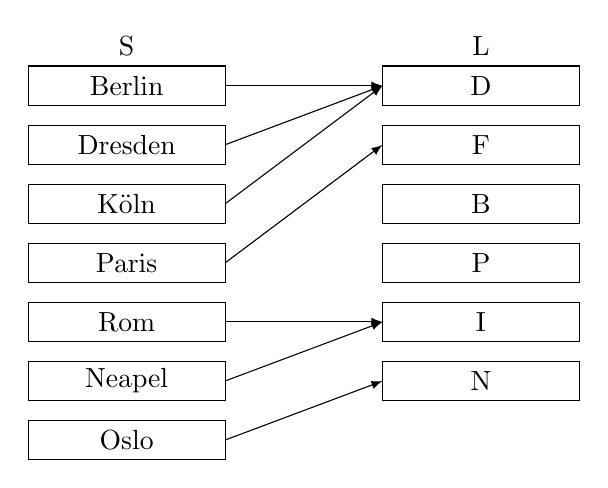
\begin{tikzpicture} [scale=0.25]

            \draw  (0,2) rectangle (10,0) node[pos =.5]{Berlin};
            \draw  (0,-1) rectangle (10,-3) node[pos =.5]{Dresden};
            \draw  (0,-4) rectangle (10,-6) node[pos =.5]{Köln};
            \draw  (0,-7) rectangle (10,-9) node[pos =.5]{Paris};
            \draw  (0,-10) rectangle (10,-12) node[pos =.5]{Rom};
            \draw  (0,-13) rectangle (10,-15) node[pos =.5]{Neapel};
            \draw  (0,-16) rectangle (10,-18) node[pos =.5]{Oslo};
            
            
            \draw  (18,2) rectangle (28,0) node[pos =.5]{D};
            \draw  (18,-1) rectangle (28,-3) node[pos =.5]{F};
            \draw  (18,-4) rectangle (28,-6) node[pos =.5]{B};
            \draw  (18,-7) rectangle (28,-9) node[pos =.5]{P};
            \draw  (18,-10) rectangle (28,-12) node[pos =.5]{I};
            \draw  (18,-13) rectangle (28,-15) node[pos =.5]{N};
            
            \node at (5,3) {S};
            \node at (23,3) {L};
            \draw[-latex] (10,1) -- (18,1);
            \draw[-latex] (10,-2) -- (18,1);
            \draw[-latex] (10,-5) -- (18,1);
            \draw[-latex] (10,-8) -- (18,-2);
            \draw[-latex] (10,-11) -- (18,-11);
            \draw[-latex] (10,-14) -- (18,-11);
            \draw[-latex] (10,-17) -- (18,-14);
        \end{tikzpicture}\\
\end{enumerate}

\paragraph{4. Definition} Eigenschaften bin"arer Relationen in $M\times M$\\
Eine Relation $T\subset M\times M$ hei"st
\begin{enumerate}[label=\alph*)]
    \item reflexiv, wenn $(x,x)\in T$ f"ur alle $x\in M$
    \item symetrisch, wenn $(x,y)\in T\Rightarrow (y,x)\in T$
    \item antisymetrisch, wenn $((x,y)\in T\land(y,x)\in T)\Rightarrow x=y$
    \item asymetrisch, wenn $(x,y)\in T\Rightarrow (y,x)\notin T$
    \item transitiv, wenn $((x,y)\in T\land (y,x)\in T)\Rightarrow (x,y)\in T$
\end{enumerate}
jeweils f"ur alle $x,y,z\in M$

\paragraph{5. Beispiel} Es sei $P$ eie Menge von Personen
\begin{enumerate}[label=\alph*)]
    \item Eine Person $x\in P$ sei j"unger als $y\in P$, wenn ihr Geburtsdatum gr"o"ser/sp"ater als das von $y$ ist. 
\end{enumerate}